\section{Auswertung}
\label{sec:auswertung}

\subsection{Bestimmung der Schallgeschwindigkeit in Acrylglas} % (fold)
\label{sub:bestimmung_der_schallgeschwindigkeit_in_acrylglas}

\begin{table}[!h]
\begin{center}
\begin{tabular}{|r|r|r|r|}
\hline
Puls-Echo & & Durchschall & \\
\hline
\hline
 L"ange[$\SI{}{\milli\meter}$] & Laufzeit[$\SI{}{\micro\second}$] & L"ange[$\SI{}{\milli\meter}$] & Laufzeit[$\SI{}{\micro\second}$]\\
\hline
\hline
 39,65 &	15,60 &	 39,65 &	16,6\\
 80,40 &	30,55 &	 80,40 &	31,7\\
120,40 &	45,15 &	120,40 &	46,4\\
\hline
\end{tabular}
\caption[]{Me"sergebnisse zur Bestimmung der Schallgeschwindigkeit in Acrylglas der 1Mhz Sonde.}
\label{a1}
\end{center}
\end{table}

\begin{table}[!h]
\begin{center}
\begin{tabular}{|r|r|}
\hline
 L"ange[$\SI{}{\milli\meter}$] & Laufzeit[$\SI{}{\micro\second}$]\\
\hline
\hline
39.65 &	15.15\\
39.65 &	15.40\\
80.40 &	30.10\\
80.40 &	30.80\\
120.4 &	44.75\\
120.4 &	45.50\\
\hline
\end{tabular}
\caption[]{Me"sergebnisse zur Bestimmung der Schallgeschwindigkeit in Acrylglas der 2Mhz Sonde.}
\label{a2}
\end{center}
\end{table}

\begin{table}[!h]
\begin{center}
\begin{tabular}{|r|r|r|r|}
\hline
Puls-Echo & & Durchschall &\\
\hline
 L"ange[$\SI{}{\milli\meter}$] & Laufzeit[$\SI{}{\micro\second}$] & L"ange[$\SI{}{\milli\meter}$] & Laufzeit[$\SI{}{\micro\second}$]\\
\hline
\hline
 39,65 &	14,85 &	 39,65 &	15,4\\
 80,40 &	29,75 &	 80,40 &	30,3\\
120,40 &	44,35 &	120,40 &	44,9\\
\hline
\end{tabular}
\caption[]{Me"sergebnisse zur Bestimmung der Schallgeschwindigkeit in Acrylglas der 4Mhz Sonde.}
\label{a4}
\end{center}
\end{table}

In den Tabellen \ref{a1}, \ref{a2} und \ref{a4} sind die Messergebnisse aufgetragen, die sich beim Puls-Echo und beim Durchschallungs Verfahren ergaben. Dabei ist zu ber"ucksichtigen, dass bei dem Puls-Echo Verfahren die Strecke und die Laufzeit halbiert wurde und daher aus Genauigkeitsgr"unden eine weitere Nachkommastelle hinzukommt.
Eine lineare Ausgleichsrechnung der Verfahren mittels $f(x) = m \cdot x + a$ ergibt die gesuchten gr"o"sen. Die Steigung $m$ gibt dabei die Schallgeschwindigkeit $v$ an. Die Verschiebung des Y-Achsenabschnitts gibt eine virtuelle L"ange des Zylinders an. Diese entspricht der zu durchlaufenden Schicht der Sonde unter der Annahme, dass in dieser die Schallgeschwindigkeit gleich der in Acrylglas ist. Somit ist der Betrag von $a$ gleich $\delta s$, was die zweifache Differenz der virtuellen mit der realen L"ange des Zylinders entspricht.

\subsubsection{1 MHz Sonde} % (fold)
\label{sub:1_mhz_sonde}

\begin{figure}[!h]
	\centering
	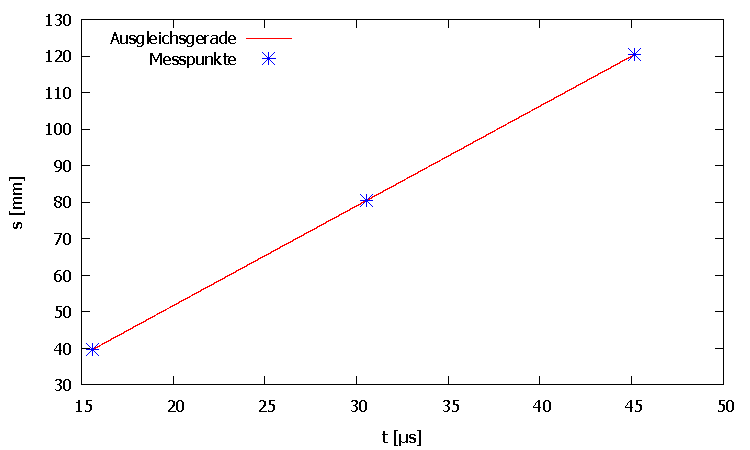
\includegraphics[width = 13cm]{img/a1e.pdf}
	\caption{Bestimmung der Schallgeschwindigkeit von Acrylglas mit dem Puls-Echo Verfahren. Dabei ist die Zeit, welche von der Schallwelle ben"otigt wird um den Zylinder einmal zu durchqueren, gegen die H"ohe des Zylinders aufgetragen.}
	\label{a1e}
\end{figure}

In Graphik \ref{a1e} sind die Ergebnisse des Puls-Echo Verfahrens aufgetragen. Es wurde eine lineare Auslgeichsrechnung durchgef"uhrt, welche zu folgenden Ergebnissen f"uhrte:

\begin{eqnarray*}
	m = v &=& \SI{2.733 (4)}{\milli\meter\per\micro\per\second}\\
	|a| = |2 \cdot \delta s| &=& |\SI{-3.0 (1)}{\milli\meter}|\\
	\delta s &=& \SI{1.51 (7)}{\milli\meter}
\end{eqnarray*}

\clearpage

\begin{figure}[!h]
	\centering
	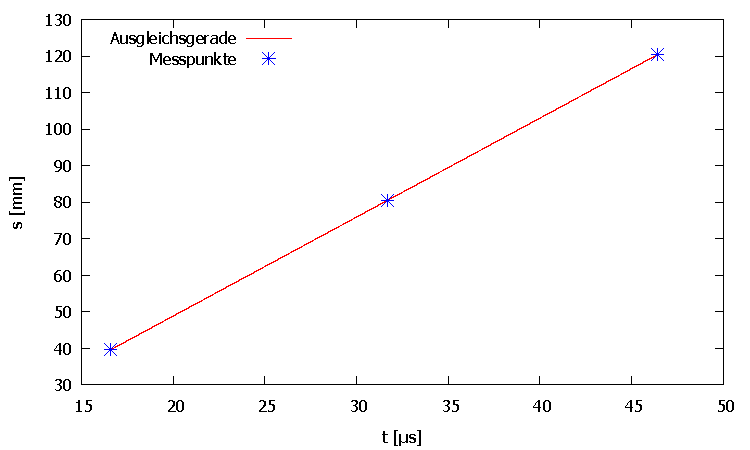
\includegraphics[width = 13cm]{img/a1d.pdf}
	\caption{Bestimmung der Schallgeschwindigkeit von Acrylglas mit dem Durchschallungs Verfahren. Dabei ist die Zeit, welche von der Schallwelle ben"otigt wird um den Zylinder einmal zu durchqueren, gegen die H"ohe des Zylinders aufgetragen.}
	\label{a1d}
\end{figure}


In Graphik \ref{a1d} sind die Ergebnisse des Durchschallungs Verfahrens aufgetragen. Es wurde eine lineare Auslgeichsrechnung durchgef"uhrt, welche zu folgenden Ergebnissen f"uhrte:

\begin{eqnarray*}
	m = v &=& \SI{2.710 (6)}{\milli\meter\per\micro\per\second}\\
	|a| = |2 \cdot \delta s| &=& |\SI{-5.39 (2)}{\milli\meter}|\\
	\delta s &=& \SI{2.7 (1)}{\milli\meter}
\end{eqnarray*}

In Tabelle \ref{r1} sind die wichtigen Gr"o"sen noch einmal zusammengefasst. $\delta t$ gibt ist dabei aus den Mittelwerten von $v$ und $\delta s$ errechnet worden. Dies ist die konstante Laufzeitkorrektur f"ur die $\SI{1}{\mega\hertz}$ Sonde, welche durch die Anpassungsschicht entsteht.

\begin{table}[!h]
\begin{center}
\begin{tabular}{|r|r|r|r|}
\hline
Puls-Echo & & Durchschall & \\
\hline
\hline
$v_\mathrm{e}$[$\SI{}{\milli\meter\per\micro\per\second}$] & $\delta$s[$\SI{}{\milli\meter}$] & $v_\mathrm{d}$[$\SI{}{\milli\meter\per\micro\per\second}$]& $\delta$s[$\SI{}{\milli\meter}$]\\
\hline
$\SI{2.733 (4)}{}$ & $\SI{3.013 (132)}{}$ & $\SI{2.710 (6)}{}$ & $\SI{5.386 (219)}{}$\\
\hline
\hline
&&&\\
$\bar{\mathrm{v}}$ & $\SI{2.721 (4)}{}$ & $\bar{\delta s}$ & $\SI{4.199 (128)}{}$\\
\hline
$\delta$t & $\SI{1.543 (47)}{}$ & &\\
\hline
\end{tabular}
\caption[]{Ergebnisse der linearen Regression f"ur die $\SI{1}{\mega\hertz}$ Sonde.}
\label{r1}
\end{center}
\end{table}

\subsubsection{2 MHz Sonde} % (fold)
\label{sub:1_mhz_sonde}

\begin{figure}[!h]
	\centering
	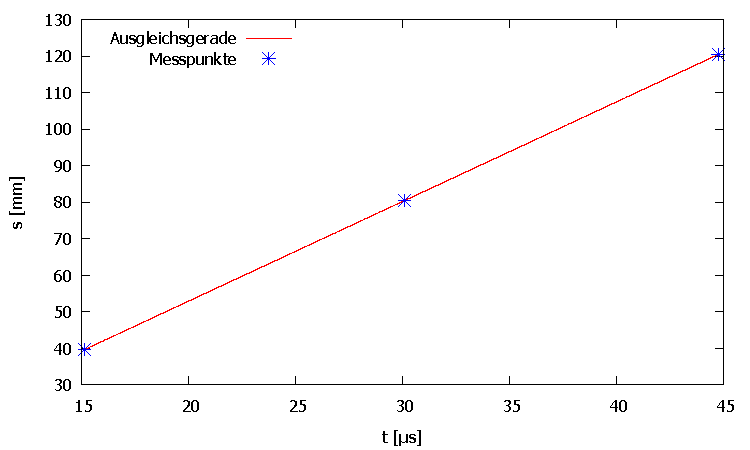
\includegraphics[width = 13cm]{img/a2e.pdf}
	\caption{Bestimmung der Schallgeschwindigkeit von Acrylglas mit dem Puls-Echo Verfahren. Dabei ist die Zeit, welche von der Schallwelle ben"otigt wird um den Zylinder einmal zu durchqueren, gegen die H"ohe des Zylinders aufgetragen.}
	\label{a2e}
\end{figure}

In Graphik \ref{a2e} sind die Ergebnisse des Puls-Echo Verfahrens aufgetragen. Es wurde eine lineare Auslgeichsrechnung durchgef"uhrt, welche zu folgenden Ergebnissen f"uhrte:

\begin{eqnarray*}
	m = v &=& \SI{2.728 (1)}{\milli\meter\per\micro\per\second}\\
	|a| = |2 \cdot \delta s| &=& |\SI{-1.69 (4)}{\milli\meter}|\\
	\delta s &=& \SI{0.85 (2)}{\milli\meter}
\end{eqnarray*}

\clearpage

\begin{figure}[!h]
	\centering
	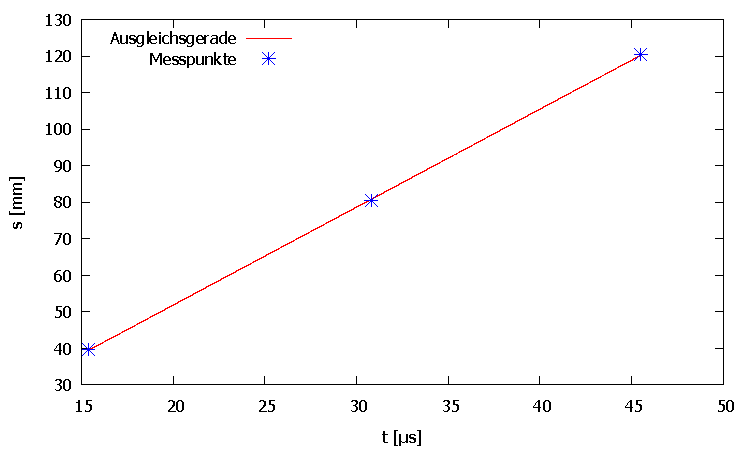
\includegraphics[width = 13cm]{img/a2d.pdf}
	\caption{Bestimmung der Schallgeschwindigkeit von Acrylglas mit dem Durchschallungs Verfahren. Dabei ist die Zeit, welche von der Schallwelle ben"otigt wird um den Zylinder einmal zu durchqueren, gegen die H"ohe des Zylinders aufgetragen.}
	\label{a2d}
\end{figure}


In Graphik \ref{a2d} sind die Ergebnisse des Durchschallungs Verfahrens aufgetragen. Es wurde eine lineare Auslgeichsrechnung durchgef"uhrt, welche zu folgenden Ergebnissen f"uhrte:

\begin{eqnarray*}
	m = v &=& \SI{2.68 (2)}{\milli\meter\per\micro\per\second}\\
	|a| = |2 \cdot \delta s| &=& |\SI{-1.8 (7)}{\milli\meter}|\\
	\delta s &=& \SI{0.9 (4)}{\milli\meter}
\end{eqnarray*}

In Tabelle \ref{r2} sind die wichtigen Gr"o"sen noch einmal zusammengefasst. $\delta t$ gibt ist dabei aus den Mittelwerten von $v$ und $\delta s$ errechnet worden. Dies ist die konstante Laufzeitkorrektur f"ur die $\SI{2}{\mega\hertz}$ Sonde, welche durch die Anpassungsschicht entsteht.

\begin{table}[!h]
\begin{center}
\begin{tabular}{|r|r|r|r|}
\hline
Puls-Echo & & Durchschall & \\
\hline
\hline
$v_\mathrm{e}$[$\SI{}{\milli\meter\per\micro\per\second}$] & $\delta$s[$\SI{}{\milli\meter}$] & $v_\mathrm{d}$[$\SI{}{\milli\meter\per\micro\per\second}$]& $\delta$s[$\SI{}{\milli\meter}$]\\
\hline
$\SI{2.728 (1)}{}$ & $\SI{1.691 (43)}{}$ & $\SI{2.682 (22)}{}$ & $\SI{1.84306 (713)}{}$\\
\hline
\hline
&&&\\
$\bar{\mathrm{v}}$[$\SI{}{\milli\meter\per\micro\per\second}$] & $\SI{2.705 (11)}{}$ & $\bar{\delta s}$[$\SI{}{\milli\meter}$] & $\SI{1.767 (357)}{}$\\
\hline
$\delta$t & $\SI{0.653 (132)}{}$ &&\\
\hline
\end{tabular}
\caption[]{Ergebnisse der linearen Regression f"ur die $\SI{2}{\mega\hertz}$ Sonde.}
\label{r2}
\end{center}
\end{table}

\subsubsection{4 MHz Sonde} % (fold)
\label{sub:1_mhz_sonde}

\begin{figure}[!h]
	\centering
	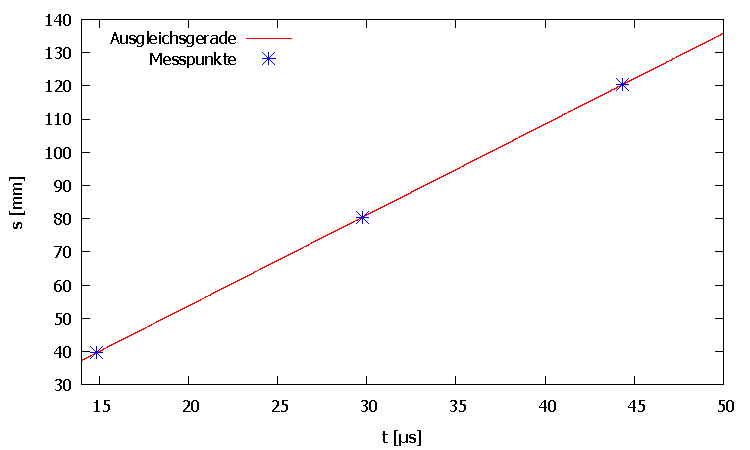
\includegraphics[width = 13cm]{img/a4e.pdf}
	\caption{Bestimmung der Schallgeschwindigkeit von Acrylglas mit dem Puls-Echo Verfahren. Dabei ist die Zeit, welche von der Schallwelle ben"otigt wird um den Zylinder einmal zu durchqueren, gegen die H"ohe des Zylinders aufgetragen.}
	\label{a4e}
\end{figure}

In Graphik \ref{a4e} sind die Ergebnisse des Puls-Echo Verfahrens aufgetragen. Es wurde eine lineare Auslgeichsrechnung durchgef"uhrt, welche zu folgenden Ergebnissen f"uhrte:

\begin{eqnarray*}
	m = v &=& \SI{2.737 (1)}{\milli\meter\per\micro\per\second}\\
	|a| = |2 \cdot \delta s| &=& |\SI{-1.01 (4)}{\milli\meter}|\\
	\delta s &=& \SI{0.51 (2)}{\milli\meter}
\end{eqnarray*}

\clearpage

\begin{figure}[!h]
	\centering
	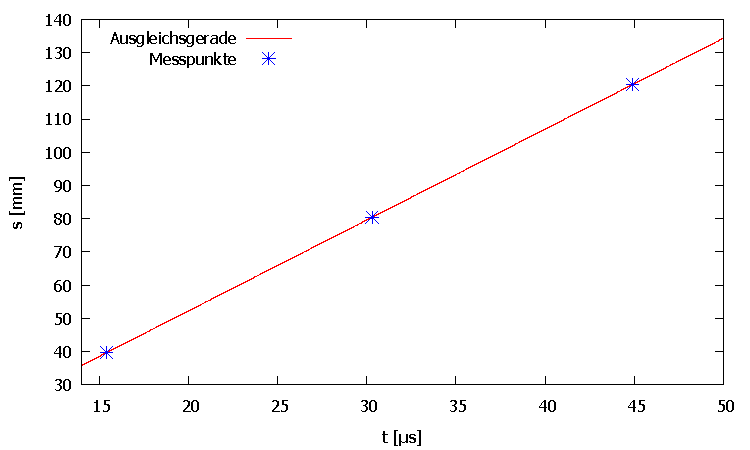
\includegraphics[width = 13cm]{img/a4d.pdf}
	\caption{Bestimmung der Schallgeschwindigkeit von Acrylglas mit dem Durchschallungs Verfahren. Dabei ist die Zeit, welche von der Schallwelle ben"otigt wird um den Zylinder einmal zu durchqueren, gegen die H"ohe des Zylinders aufgetragen.}
	\label{a4d}
\end{figure}


In Graphik \ref{a4d} sind die Ergebnisse des Durchschallungs Verfahrens aufgetragen. Es wurde eine lineare Auslgeichsrechnung durchgef"uhrt, welche zu folgenden Ergebnissen f"uhrte:

\begin{eqnarray*}
	m = v &=& \SI{2.737 (1)}{\milli\meter\per\micro\per\second}\\
	|a| = |2 \cdot \delta s| &=& |\SI{-2.52 (5)}{\milli\meter}|\\
	\delta s &=& \SI{1.26 (2)}{\milli\meter}
\end{eqnarray*}

In Tabelle \ref{r4} sind die wichtigen Gr"o"sen noch einmal zusammengefasst. $\delta t$ gibt ist dabei aus den Mittelwerten von $v$ und $\delta s$ errechnet worden. Dies ist die konstante Laufzeitkorrektur f"ur die $\SI{4}{\mega\hertz}$ Sonde, welche durch die Anpassungsschicht entsteht.

\begin{table}[!h]
\begin{center}
\begin{tabular}{|r|r|r|r|}
\hline
Puls-Echo & & Durchschall & \\
\hline
\hline
v[$\SI{}{\milli\meter\per\micro\per\second}$] & $\delta$s[$\SI{}{\milli\meter}$] & v[$\SI{}{\milli\meter\per\micro\per\second}$]& $\delta$s[$\SI{}{\milli\meter}$]\\
\hline
$\SI{2.737 (1)}{}$ & $\SI{1.010 (44)}{}$ & $\SI{2.737 (1)}{}$ & $\SI{2.516 (45)}{}$\\
\hline
\hline
\\
$\bar{\mathrm{v}}$[$\SI{}{\milli\meter\per\micro\per\second}$] & $\SI{2.737 (1)}{}$ & $\bar{\delta s}$[$\SI{}{\milli\meter}$] & $\SI{1.763 (32)}{}$\\
\hline
\end{tabular}
\caption[]{Ergebnisse der linearen Regression f"ur die $\SI{4}{\mega\hertz}$ Sonde.}
\label{r4}
\end{center}
\end{table}


\subsection{Bestimmung der Lochbreite im Acrylglas} % (fold)
\label{sub:bestimmung_der_lochbreite_im_acrylglas}


\begin{table}[!h]
\begin{center}
\begin{tabular}{|r|r|r|r|r|r|}
\hline
 $\SI{1}{\mega\hertz}$ && $\SI{2}{\mega\hertz}$ && $\SI{3}{\mega\hertz}$&\\
\hline
Peak1[$\SI{}{\micro\second}$] & Peak2[$\SI{}{\micro\second}$] & Peak1[$\SI{}{\micro\second}$] & Peak2[$\SI{}{\micro\second}$] & Peak1[$\SI{}{\micro\second}$] & Peak2[$\SI{}{\micro\second}$]\\
\hline
\hline
42.1 &	13.2 &	40.9 &	12.2 &	40.6 &	11.8\\
12.2 &	48.2 &	11.2 &	47.1 &	10.9 &	46.6\\
18.2 &	42.3 &	17.1 &	41.2 &	16.7 &	40.7\\
24.1 &	36.4 &	23.0 &	35.3 &	22.6 &	34.8\\
30.1 &	30.5 &	29.0 &	29.3 &	28.5 &	28.9\\
35.5 &	24.4 &	34.4 &	23.2 &	33.9 &	22.8\\
41.2 &	18.0 &	40.0 &	16.8 &	39.5 &	16.4\\
46.5 &	11.7 &	45.5 &	10.7 &	45.0 &	10.4\\
15.0 &	46.3 &	14.0 &	45.6 &	13.6 &	45.1\\
16.1 &	45.5 &	15.3 &	44.4 &	14.9 &	43.8\\
\hline
\end{tabular}
\caption[]{Durch das Puls-Echo Verfahren erhaltene Werte zur Bestimmung der Lochgr"o"se.}
\label{loch1}
\end{center}
\end{table}

Die H"ohe der gest"orten Probe betr"agt:

\begin{equation*}
	h = \SI{79.7 (2)}{\milli\meter}
\end{equation*}

In Tabelle \ref{loch} sind die gemessen Werte zur Bestimmung der Breite der St"orstellen nach \ref{sec:durchfuehrung} Abb. \ref{fig:klotz} in Acrylglas aufgelistet. Es ist zu beachten, dass die Breite der St"orstelle 10 nicht untersucht werden konnte, da diese nur von einer Seite beschallt werden konnte. Zu erkl"aren ist dies, weil diese im Schatten der sehr viel gr"o"seren St"orstelle 11 liegt.

Zur Bestimmung der Breite ist es zun"achst notwendig die Strecke von beiden Seiten zur St"orstelle zu ermitteln.
Da dies mit Impuls-Echo Verfahren durchgef"uhrt wird, muss die Zeit $t$ halbiert werden. Diese entspricht nun der Zeit, welche zum Erreichen der St"orstelle gebraucht wird.
Aus den zuvor ermittelten Schallgeschwindigkeiten f"ur die einzelnen Sonden l"asst sich daraus die Strecke nach Gleichung \eqref{s1} berechnen. Nun muss noch die L"ange $\delta s$ abgezogen werden, da diese dem Weg in der Sonde entspricht. Das gleiche wird mit den Ergebnissen auf der R"uckseite durchgef"uhrt. Nun gilt f"ur die Breite der St"orstellen:

\begin{eqnarray*}
	b &=& h - (d_\mathrm{hin} - d_\mathrm{r"uck})\\
	\Delta  b &=& = \sqrt{\left(\Delta h \right)^2 + (\Delta s_\mathrm{1})^2 + (\Delta s_\mathrm{2})^2}\\
	\Delta s_\mathrm{1,2} &=& \sqrt{(\Delta s_\mathrm{eff,1,2})^2 + (\Delta \delta s)^2}\\
	\Delta s_\mathrm{eff,1,2} &=& \frac{1}{2} t \Delta v
\end{eqnarray*}

\subsubsection{1 MHz Sonde} % (fold)
\label{sub:1_mhz_sonde}

\begin{table}[!h]
\begin{center}
\begin{tabular}{|r|r|r|r|r|r|}
\hline
$\frac{1}{2}t_\mathrm{1}[\SI{}{\micro\second}$] & $\frac{1}{2}t_\mathrm{2}[\SI{}{\micro\second}$] & $s_\mathrm{eff,1}[\SI{}{\milli\meter}]$ & $\Delta s_\mathrm{eff,1}[\SI{}{\milli\meter}]$ & $s_\mathrm{eff,2}[\SI{}{\milli\meter}]$ & $\Delta s_\mathrm{eff,2}[\SI{}{\milli\meter}]$ \\ 
\hline
\hline
21.05 &	 6.60 &	57.28 &	0.08 &	17.95 &	0.02 \\
 6.10 &	24.10 &	16.59 &	0.02 &	65.57 &	0.09 \\
 9.10 &	21.15 &	24.76 &	0.03 &	57.55 &	0.08 \\
12.05 &	18.20 &	32.78 &	0.04 &	49.52 &	0.06 \\
15.05 &	15.25 &	40.95 &	0.05 &	41.49 &	0.05 \\
17.75 &	12.20 &	48.30 &	0.06 &	33.19 &	0.04 \\
20.60 &	 9.00 &	56.05 &	0.07 &	24.49 &	0.03 \\
23.25 &	 5.85 &	63.26 &	0.08 &	15.91 &	0.02 \\
 7.50 &	23.15 &	20.40 &	0.02 &	62.99 &	0.08 \\
 8.05 &	22.75 &	21.90 &	0.03 &	61.90 &	0.08 \\
 \hline
 \hline
$s_\mathrm{1}[\SI{}{\milli\meter}]$ & $\Delta s_\mathrm{1}[\SI{}{\milli\meter}]$ & $s_\mathrm{2}[\SI{}{\milli\meter}]$ & $\Delta s_\mathrm{2}[\SI{}{\milli\meter}]$ & b[$\SI{}{\milli\meter}$] & $\Delta$b[$\SI{}{\milli\meter}$]\\
\hline
\hline
55.18 &	0.10 &	15.85 &	0.06 &	8.66 &	0.24\\
14.49 &	0.06 &	63.48 &	0.11 &	1.72 &	0.24\\
22.66 &	0.07 &	55.45 &	0.10 &	1.58 &	0.24\\
30.69 &	0.07 &	47.42 &	0.09 &	1.58 &	0.23\\
38.85 &	0.08 &	39.39 &	0.08 &	1.45 &	0.23\\
46.20 &	0.09 &	31.09 &	0.07 &	2.40 &	0.23\\
53.95 &	0.10 &	22.39 &	0.07 &	3.35 &	0.24\\
61.16 &	0.10 &	13.81 &	0.06 &	4.71 &	0.24\\
18.30 &	0.06 &	60.89 &	0.10 &	0.50 &	0.24\\
19.80 &	0.07 &	59.80 &	0.10 &	0.09 &	0.24\\
\hline
\end{tabular}
\caption[]{Daten zur Bestimmung der Lochbreiten b mit einer $\SI{1}{\mega\hertz}$ Sonde. Dabei ist $s_\mathrm{eff}$ die Strecke inklusive des Sondenwegs, $s$ die Strecke ohne Sondenweg, $t$ die Laufzeit und $b$ die Lochbreite.}
\label{loch1}
\end{center}
\end{table}

In Tabelle \ref{loch1} sind die Breiten der St"orstellen, sowie die zur Berechnung ben"otigten Werte aufgelistet. Hierbei konnte besonders gut weiter entfernte St"orstellen und die R"uckwand erkannt werden. Dabei geht jedoch die Sch"arfe verloren.

\clearpage
\subsubsection{2 MHz Sonde} % (fold)
\label{sub:1_mhz_sonde}

\begin{table}[!h]
\begin{center}
\begin{tabular}{|r|r|r|r|r|r|}
\hline
$\frac{1}{2}t_\mathrm{1}[\SI{}{\micro\second}$] & $\frac{1}{2}t_\mathrm{2}[\SI{}{\micro\second}$] & $s_\mathrm{eff,1}[\SI{}{\milli\meter}]$ & $\Delta s_\mathrm{eff,1}[\SI{}{\milli\meter}]$ & $s_\mathrm{eff,2}[\SI{}{\milli\meter}]$ & $\Delta s_\mathrm{eff,2}[\SI{}{\milli\meter}]$ \\ 
\hline
\hline
21.05 &	 6.60 &	55.32 &	0.23 &	16.50 &	0.07 \\
 6.10 &	24.10 &	15.15 &	0.07 &	63.71 &	0.26 \\
 9.10 &	21.15 &	23.13 &	0.10 &	55.73 &	0.23 \\
12.05 &	18.20 &	31.11 &	0.13 &	47.75 &	0.20 \\
15.05 &	15.25 &	39.23 &	0.16 &	39.63 &	0.17 \\
17.75 &	12.20 &	46.53 &	0.19 &	31.38 &	0.13 \\
20.60 &	 9.00 &	54.10 &	0.22 &	22.72 &	0.10 \\
23.25 &	 5.85 &	61.54 &	0.25 &	14.47 &	0.06 \\
 7.50 &	23.15 &	18.94 &	0.08 &	61.68 &	0.25 \\
 8.05 &	22.75 &	20.70 &	0.09 &	60.06 &	0.25 \\
 \hline
 \hline
$s_\mathrm{1}[\SI{}{\milli\meter}]$ & $\Delta s_\mathrm{1}[\SI{}{\milli\meter}]$ & $s_\mathrm{2}[\SI{}{\milli\meter}]$ & $\Delta s_\mathrm{2}[\SI{}{\milli\meter}]$ & b[$\SI{}{\milli\meter}$] & $\Delta$b[$\SI{}{\milli\meter}$]\\
\hline
\hline
54.44 &	0.42 &	15.62 &	0.36 &	9.64 &	0.59\\
14.27 &	0.36 &	62.82 &	0.44 &	2.61 &	0.61\\
22.25 &	0.37 &	54.84 &	0.42 &	2.61 &	0.60\\
30.23 &	0.38 &	46.86 &	0.41 &	2.61 &	0.59\\
38.34 &	0.39 &	38.75 &	0.39 &	2.61 &	0.59\\
45.65 &	0.41 &	30.50 &	0.38 &	3.56 &	0.59\\
53.22 &	0.42 &	21.84 &	0.37 &	4.64 &	0.60\\
60.66 &	0.44 &	13.59 &	0.36 &	5.45 &	0.60\\
18.05 &	0.37 &	60.80 &	0.44 &	0.85 &	0.60\\
19.81 &	0.37 &	59.17 &	0.43 &	0.72 &	0.60\\
\hline
\end{tabular}
\caption[]{Daten zur Bestimmung der Lochbreite b mit einer $\SI{2}{\mega\hertz}$ Sonde. Dabei ist $s_\mathrm{eff}$ die Strecke inklusive des Sondenwegs, $s$ die Strecke ohne Sondenweg, $t$ die Laufzeit und $b$ die Lochbreite.}
\label{loch1}
\end{center}
\end{table}

In Tabelle \ref{loch2} sind die Breiten der St"orstellen, sowie die zur Berechnung ben"otigten Werte aufgelistet. Bei diesem Verfahren konnten sowohl nahe als auch weiter entfernte St"orstellen relativ scharf dargestellt werden.

\clearpage
\subsubsection{4 MHz Sonde} % (fold)
\label{sub:1_mhz_sonde}

\begin{table}[!h]
\begin{center}
\begin{tabular}{|r|r|r|r|r|r|}
\hline
$\frac{1}{2}t_\mathrm{1}[\SI{}{\micro\second}$] & $\frac{1}{2}t_\mathrm{2}[\SI{}{\micro\second}$] & $s_\mathrm{eff,1}[\SI{}{\milli\meter}]$ & $\Delta s_\mathrm{eff,1}[\SI{}{\milli\meter}]$ & $s_\mathrm{eff,2}[\SI{}{\milli\meter}]$ & $\Delta s_\mathrm{eff,2}[\SI{}{\milli\meter}]$ \\ 
\hline
\hline
21.05 &	 6.60 &	55.57 &	0.03 &	16.15 &	0.01 \\
 6.10 &	24.10 &	14.92 &	0.01 &	63.78 &	0.03 \\
 9.10 &	21.15 &	22.86 &	0.01 &	55.70 &	0.03 \\
12.05 &	18.20 &	30.93 &	0.02 &	47.63 &	0.02 \\
15.05 &	15.25 &	39.01 &	0.02 &	39.55 &	0.02 \\
17.75 &	12.20 &	46.40 &	0.02 &	31.20 &	0.02 \\
20.60 &	 9.00 &	54.06 &	0.03 &	22.45 &	0.01 \\
23.25 &	 5.85 &	61.59 &	0.03 &	14.23 &	0.01 \\
 7.50 &	23.15 &	18.61 &	0.01 &	61.73 &	0.03 \\
 8.05 &	22.75 &	20.39 &	0.01 &	59.95 &	0.03 \\
 \hline
 \hline
$s_\mathrm{1}[\SI{}{\milli\meter}]$ & $\Delta s_\mathrm{1}[\SI{}{\milli\meter}]$ & $s_\mathrm{2}[\SI{}{\milli\meter}]$ & $\Delta s_\mathrm{2}[\SI{}{\milli\meter}]$ & b[$\SI{}{\milli\meter}$] & $\Delta$b[$\SI{}{\milli\meter}$]\\
\hline
\hline
54.69 &	0.04 &	15.27 &	0.03 &	9.75 &	0.21\\
14.04 &	0.03 &	62.90 &	0.05 &	2.77 &	0.21\\
21.97 &	0.03 &	54.82 &	0.04 &	2.90 &	0.21\\
30.05 &	0.04 &	46.75 &	0.04 &	2.90 &	0.21\\
38.12 &	0.04 &	38.67 &	0.04 &	2.90 &	0.21\\
45.52 &	0.04 &	30.32 &	0.04 &	3.86 &	0.21\\
53.18 &	0.04 &	21.56 &	0.03 &	4.96 &	0.21\\
60.71 &	0.04 &	13.35 &	0.03 &	5.64 &	0.21\\
17.73 &	0.03 &	60.84 &	0.04 &	1.12 &	0.21\\
19.51 &	0.03 &	59.06 &	0.04 &	1.12 &	0.21\\
\hline
\end{tabular}
\caption[]{Daten zur Bestimmung der Lochbreiten b mit einer $\SI{4}{\mega\hertz}$ Sonde. Dabei ist $s_\mathrm{eff}$ die Strecke inklusive des Sondenwegs, $s$ die Strecke ohne Sondenweg, $t$ die Laufzeit und $b$ die Lochbreite.}
\label{loch4}
\end{center}
\end{table}

In Tabelle \ref{loch4} sind die Breiten der St"orstellen, sowie die zur Berechnung ben"otigten Werte aufgelistet. Weiter entfernte St"orstellen waren nicht mehr gut messbar, doch nahe St"orstellen wurden besonders scharf dargestellt.

\clearpage

\subsection{B-Scan einer gest"orten Probe} % (fold)
\label{sub:b_scan_einer_gest_orten_probe}

\begin{figure}[!h]
	\centering
	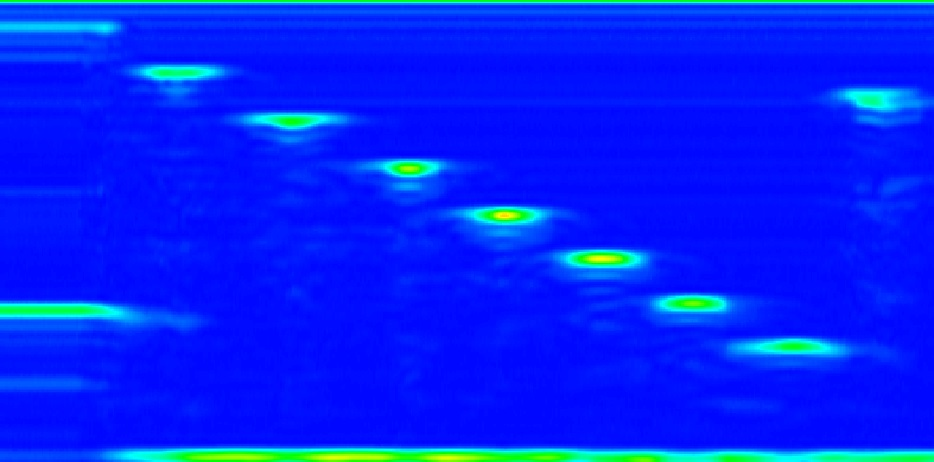
\includegraphics[width = 10.5cm]{img/1MHZ.jpg}
	\caption{B-Scan der gest"orten Probe mit einer $\SI{1}{\mega\hertz}$ Sonde.}
	\label{b1}
\end{figure}

\begin{figure}[!h]
	\centering
	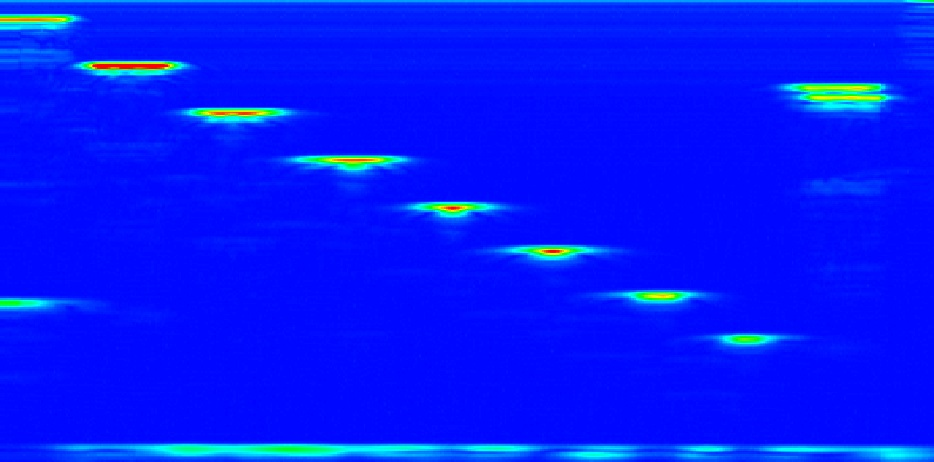
\includegraphics[width = 10.5cm]{img/2MHZ.jpg}
	\caption{B-Scan der gest"orten Probe mit einer $\SI{2}{\mega\hertz}$ Sonde.}
	\label{b2}
\end{figure}

\begin{figure}[!h]
	\centering
	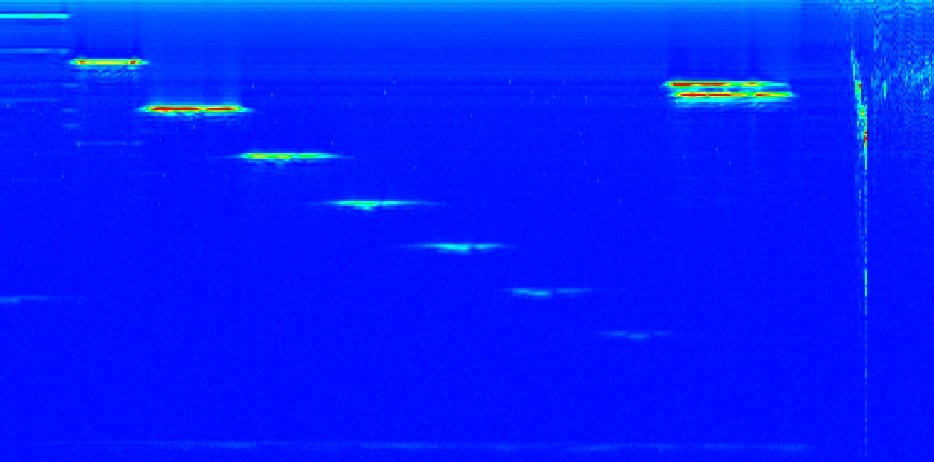
\includegraphics[width = 10.5cm]{img/4MHZ.jpg}
	\caption{B-Scan der gest"orten Probe mit einer $\SI{4}{\mega\hertz}$ Sonde.}
	\label{b4}
\end{figure}

Es ist zu erkennen, dass die Reichweite der Ultraschallwelle mit zunehmender Frequenz abnimmt. Jedoch nimmt auch die Sch"arfe der dargestellten St"orstellen zu. Es kann gesagt werden, dass hohe Frequenzen zwar weniger tief eindringen, doch im nahen Bereich eine sehr gute Aufl"osung erreichen, w"ahrend mit weniger hohen Frequenzen mehr ein gesamt"uberblick erreicht wird, doch keine genauen Aussagen getroffen werden k"onnen.

\subsection{Abmessungen eines Auges} % (fold)
\label{sub:das_auge}

\begin{table}[!h]
\begin{center}
\begin{tabular}{|r|r|r|r|r|}
\hline
Sonde[$\SI{}{\mega\hertz}$] & Peak1[$\SI{}{\micro\second}$] & Peak2[$\SI{}{\micro\second}$] & Peak3[$\SI{}{\micro\second}$] & Peak4[$\SI{}{\micro\second}$]\\
\hline
\hline
1 &	12.4 &	18.3 &	26.3 &	72.8\\
2 &	12.0 &	17.6 &	24.4 &	71.7\\
4 &	11.7 &	16.6 &	24.8 &	71.1\\
\hline
\end{tabular}
\caption[]{Messdaten zur Berechnung der Ma"se der Nachbildung eines Auges.}
\label{auge1}
\end{center}
\end{table}

In Tabelle \ref{auge1} sind die Messdaten des Auges aufgelistet.

Die Schallgeschwindigkeiten in der Linse $v_\mathrm{L}$ und dem Rest $v_\mathrm{GK}$ des Auges betr"agt:

\begin{eqnarray*}
	v_\mathrm{L} = \SI{2.5}{\milli\meter\per\micro\per\second}\\
	v_\mathrm{GK} = \SI{1.41}{\milli\meter\per\micro\per\second}
\end{eqnarray*}

Bei dieser Methode muss zun"achst die Laufzeitkorrektur $2 \delta t$ von den gemessenen Zeiten abgezogen werden.
Um den Abstand zwischen Sonde und Iris zu berechnen, muss nun die neue Zeit durch zwei geteilt werden und diese mit $v_\mathrm{GK}$ multipliziert werden.

Bei den weiteren Abst"anden wird die, f"ur den vorherigen Abstand, gemessene Zeit von der nun ben"otigten Zeit abgezogen. Es bleibt die Zeit "ubrig, welche die Welle ben"otigt um von dem vorherigen Me"spunkt wieder an diesen zur"uckzukehren. Diese Zeit durch zwei geteilt und mit der dort wirkenden Geschwindigkeit multipliziert ergibt nun den gesuchten Abstand.

Die Abst"ande der einzelnen Messbereiche sind in Tabelle \ref{loch2} augelistet.
\clearpage

\begin{table}[!h]
\begin{center}
\begin{tabular}{|r|r|r|r|r|r|}
\hline
Sonde[$\SI{}{\mega\hertz}$] & $d_\mathrm{S,I}[\SI{}{\milli\meter}]$ & $d_\mathrm{I,L1}[\SI{}{\milli\meter}]$ & $d_\mathrm{L1,L2}[\SI{}{\milli\meter}]$ & $d_\mathrm{L2,R}[\SI{}{\milli\meter}]$ & $d_\mathrm{ges}[\SI{}{\milli\meter}]$\\
\hline
\hline
1 &	7.66 &	4.16 &	10.00 & 32.78 &	54.60\\
2 & 8.00 &	3.95 &	 8.50 &	33.35 &	53.80\\
4 &	7.79 &	3.45 &	10.25 & 32.64 &	54.13\\
\hline
\end{tabular}
\caption[]{Abmessungen des Auges mithilfe verschiedener Ultraschallsonden. Dabei ist $d_\mathrm{S,I}$ der Abstand zwischen Sonde und Iris, $d_\mathrm{I,L1}$ der Abstand zwischen Iris und Linse1, $d_\mathrm{L1,L2}$ der Abstand zwischen Anfang der Linse und Ende der Linse, $d_\mathrm{L2,R}$ der Abstand zwischen Ende der Linse und der Retina.}
\label{auge2}
\end{center}
\end{table}

